% Hlavicka pro protokoly z fyzikalniho praktika.
% Verze pro: LaTeX
% Verze hlavicky: 22. 2. 2007
% Autor: Ustav fyziky kondenzovanych latek
% Ke stazeni: www.physics.muni.cz/ufkl/Vyuka/
% Licence: volne k pouziti, nejlepe k vcasnemu odevzdani protokolu z Vaseho mereni.

\documentclass[a4paper,11pt]{article}

% Kodovani (cestiny) v dokumentu: utf-8
%\usepackage[cp1250]{inputenc}	% Omezena stredoevropska kodova stranka, pouze MSW.
\usepackage[utf8]{inputenc}	% Doporucujeme pouzivat UTF-8 (unicode).

%%% Nemente:
\usepackage[margin=2cm]{geometry}
\newtoks\jmenopraktika \newtoks\jmeno \newtoks\datum
\newtoks\obor \newtoks\skupina \newtoks\rocnik \newtoks\semestr
\newtoks\cisloulohy \newtoks\jmenoulohy
\newtoks\tlak \newtoks\teplota \newtoks\vlhkost
\usepackage{amsmath}
\usepackage{mathtools}
\usepackage{graphicx}
\usepackage{multirow}
\graphicspath{ {./images/} }
%%% Nemente - konec.


%%%%%%%%%%% Doplnte pozadovane polozky:

\jmenopraktika={Fyzikální praktikum 2}  % nahradte jmenem vaseho predmetu
\jmeno={Artem Gorodilov}            % nahradte jmenem mericiho
\datum={2. ~listopadu  2023}        % nahradte datem mereni ulohy
\obor={Astrofyzika}                     % nahradte zkratkou vami studovaneho oboru
\skupina={Čt 8:00}            % nahradte dobou vyuky vasi seminarni skupiny
\rocnik={II}                  % nahradte rocnikem, ve kterem studujete
\semestr={I}                 % nahradte semestrem, ve kterem studujete

\cisloulohy={7}               % nahradte cislem merene ulohy
\jmenoulohy={Odraz a lom světla. Fresnelovy vztahy, Snellův zákon} % nahradte jmenem merene ulohy

\tlak={979}                   % nahradte tlakem pri mereni (v hPa)
\teplota={21.4}               % nahradte teplotou pri mereni (ve stupnich Celsia)
\vlhkost={46}               % nahradte vlhkosti vzduchu pri mereni (v %)

%%%%%%%%%%% Konec pozadovanych polozek.


%%%%%%%%%%% Uzitecne balicky:
\usepackage[czech]{babel}
\usepackage{graphicx}
\usepackage{amsmath}
\usepackage{xspace}
\usepackage{url}
\usepackage{indentfirst}
\usepackage{listings}
\usepackage{subcaption}
\usepackage{caption}
\usepackage{tabularx}
\usepackage[labelformat=parens,labelsep=quad,skip=3pt]{caption}

%%%%%% Zamezeni parchantu:
\widowpenalty 10000 \clubpenalty 10000 \displaywidowpenalty 10000
%%%%%% Parametry pro moznost vsazeni vetsiho poctu obrazku na stranku
\setcounter{topnumber}{3}	  % max. pocet floatu nahore (specifikace t)
\setcounter{bottomnumber}{3}	  % max. pocet floatu dole (specifikace b)
\setcounter{totalnumber}{6}	  % max. pocet floatu na strance celkem
\renewcommand\topfraction{0.9}	  % max podil stranky pro floaty nahore
\renewcommand\bottomfraction{0.9} % max podil stranky pro floaty dole
\renewcommand\textfraction{0.1}	  % min podil stranky, ktery musi obsahovat text
\intextsep=8mm \textfloatsep=8mm  %\intextsep pro ulozeni [h] floatu a \textfloatsep pro [b] or [t]

% Tecky za cisly sekci:
\renewcommand{\thesection}{\arabic{section}.}
\renewcommand{\thesubsection}{\thesection\arabic{subsection}.}
% Jednopismenna mezera mezi cislem a nazvem kapitoly:
\makeatletter \def\@seccntformat#1{\csname the#1\endcsname\hspace{1ex}} \makeatother

\begin{document}

\thispagestyle{empty}

{
\begin{center}
\sf 
{\Large Ústav fyzikální elektroniky PřF MU} \\
\bigskip
{\huge \bfseries FYZIKÁLNÍ PRAKTIKUM} \\
\bigskip
{\Large \the\jmenopraktika}
\end{center}

\bigskip

\sf
\noindent
\setlength{\arrayrulewidth}{1pt}
\begin{tabular*}{\textwidth}{@{\extracolsep{\fill}} l l}
\large {\bfseries Zpracoval:}  \the\jmeno & \large  {\bfseries Naměřeno:} \the\datum\\[2mm]
\large  {\bfseries Obor:} \the\obor  \hspace{40mm}  {\bfseries Skupina:} \the\skupina %
%{\bfseries Ročník:} \the\rocnik \hspace{5mm} {\bfseries Semestr:} \the\semestr  
&\large {\bfseries Testováno:}\\
\\
\hline
\end{tabular*}
}

\bigskip

{
\sf
\noindent \begin{tabular}{p{3cm} p{0.6\textwidth}}
\Large  Úloha č. {\bfseries \the\cisloulohy:} \par
\smallskip
$T=\the\teplota$~$^\circ$C \par
$p=\the\tlak$~hPa \par
$\varphi=\the\vlhkost$~\%
&\Large \bfseries \the\jmenoulohy  \\[2mm]
\end{tabular}
}

\vskip1cm
    \begin{minipage}[t]{0.5\textwidth} 
    \section{Zadání}
    Změřit odraz $S$ a $P$ polarizovaného světla od dielektrika.
    \par Zjistit Brüstedův úhel a použít jej k určení indexu lomu a porovnat naměřenou závislost na úhlu dopadu paprsku s vypočtenými hodnotami.
    \par Změřit posun paprsku při průchodu rovinnou deskou a ze závislosti posunu na úhlu dopadu určit index lomu desky.
    \section{Teorie}
        \subsection{Odraz a lom světla}
            V této úloze zkoumáme závislost složek polarizovaného světla $S$ a $P$ na úhlu dopadu. Během měření úzký svazek paprsků prochází polarizátorem. Otáčením polarizátoru můžeme měnit světlo na $S$ a $P$ složky. $P$ složka má kmitovou rovinu rovnoběžnou s rovinou dopadu, zatímco při kolmé kmitové rovině hovoříme o polarizaci $S$. Měření probíhá ve stolové soustavě, která obsahuje otáčivý stoleček kolem svislé osy, umožňující měření úhlu dopadu polarizovaného světla na dielektrikum. Po odrazu dopadá polarizované světlo na detektor, který též rotuje kolem svislé osy. Detektor měří foto-napětí, převádějící intenzitu dopadajícího světla na napětí. Fotonapětí $U_{s0}$ a $U_{p0}$ zjistíme, ponecháme-li polarizované světlo přímo dopadnout na detektor a zaznamenáme hodnoty napětí, které přímo odpovídají intenzitám $I_s^0$ a $I_p^0$.
    \end{minipage}
    \hspace{10pt}
    \begin{minipage}[t]{0.5\textwidth} 
            Reflexe pro $S$ a $P$ složky amplitudy polarizovaného světla spočítáme pomocí vzorců:
            \begin{minipage}[t]{0.45\textwidth} 
                \begin{equation}
                    R_s = \frac{I_s^R}{I_s^0}
                \end{equation}
            \end{minipage}
            \begin{minipage}[t]{0.45\textwidth} 
                \begin{equation}
                    R_p = \frac{I_p^R}{I_p^0}
                \end{equation}
            \end{minipage}
            \vspace{10pt}
            \par kde $R_s$ a $R_p$ jsou odrazivosti v rovinách $S$ a $P$ resp., $I_s^R$ a $I_p^R$ jsou intenzity odrazu světla v rovinách $S$ a $P$ resp. a $I_s^0$ a $I_p^0$ jsou již zmíněné veličiny.
            \par Intenzitu nepolarizovaného světla zjistíme podle vzorce: 
            \begin{equation}
                I = \frac{I_s^R + I_p^R}{2}
            \end{equation}
            Odrazivost nepolarizovaného světla lze zjistit podle vzorce: 
            \begin{equation}
                R = \frac{R_s + R_p}{2}
            \end{equation}
            Určuje se tzv. Brewstedův úhel $\varphi_B$, který představuje polarizační úhel dopadu. Při dosažení tohoto úhlu dochází k odrazu pouze s polarizovanými složkami světla. S narůstajícím úhlem dopadu $\varphi$ klesá hodnota $I_p^R$ na nulu, až dosáhne nuly právě v okamžiku $\varphi_B$. Po překročení úhlu $\varphi_B$ začíná $I_p^R$ opět stoupat. Naopak $I_s^R$ monotónně roste s rostoucím úhlem $\varphi$. 
            \par Index lomu dielektrika $n$ lze vypočítat pomocí Brewsterova úhlu prostřednictvím uvedeného vztahu:
            \begin{equation}
                n = tan\varphi_B ~~,~~ pokud~n_0 = 1
            \end{equation}
            kde $n_0$ je intenzita okolního světla.
    \end{minipage}
\newpage
    \begin{minipage}[t]{0.5\textwidth} 
            Index lomu dielektrika lze také vypočítat z úhlu kolem Brewsterova úhlu:
            \begin{equation}
                n = \sqrt{\frac{(1+\sqrt{R_s})(1+\sqrt{R_p})}{(1-\sqrt{R_s})(1-\sqrt{R_p})}} ~~,~~ pro~ \varphi <  \varphi_B
            \end{equation}
            \begin{equation}
                n = \sqrt{\frac{(1+\sqrt{R_s})(1-\sqrt{R_p})}{(1-\sqrt{R_s})(1+\sqrt{R_p})}} ~~,~~ pro~ \varphi >  \varphi_B
            \end{equation}
            Určit hodnotu odrazivosti, vypočítat ze vzorce pro Fresnerovy amplitudy:
            \begin{equation}
                R_s = \left\vert -\frac{sin(\varphi_0 - \varphi_1)}{sin(\varphi_0 + \varphi_1)} \right\vert^2
            \end{equation}
            \begin{equation}
                R_p = \left\vert -\frac{tan(\varphi_0 - \varphi_1)}{tan(\varphi_0 + \varphi_1)} \right\vert^2
            \end{equation}
            kde $\varphi_0$ je úhel dopadu a $\varphi_1$ je úhel odrazu, který se zjistí ze Snellova vztahu:
            \begin{equation}
                sin\varphi_1 = \frac{n_0 sin\varphi_0}{n_1}
            \end{equation}
        \subsection{Průchod světla plexisklem a sklem}
            Při průchodu světla sklem či plexisklem dochází k odchylce vstupujícího paprsku ve srovnání s paprskem dopadajícím. Pozorujeme úhlovou odchylku vstupujícího a vystupujícího paprsku, na základě které můžeme stanovit index lomu skla nebo plexiskla v prostředí s indexem lomu $n_0$.
            \par Tuto situaci popisuje obrázek (\ref{fig:scheme}).
            \vspace{10pt}
            \par \centering
            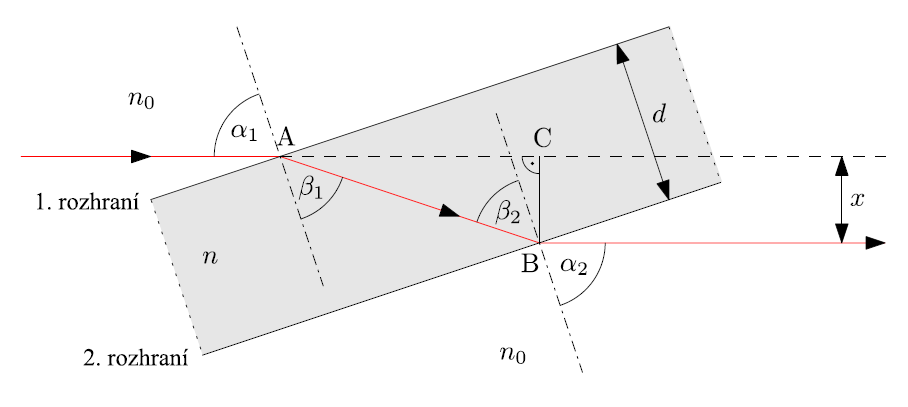
\includegraphics[scale=0.33]{scheme}
            \captionsetup{justification=centering, font=footnotesize}
            \captionof{figure}{Průchod světla planparalelní deskou.}
            \label{fig:scheme}
            \vspace{10pt}
            \raggedright
            \vspace{10pt}
            \par Poté, co paprsek vstoupí do rovinné vrstvy, jak je znázorněno na obrázku, platí zákon lomu:
            \begin{equation}
                n_0 sin \alpha = n sin \beta ~~,~~ na~prvním~rozhraní~~
            \end{equation}
            \begin{equation}
                n sin \beta = n_0 sin \alpha ~~,~~ na~druhém~rozhraní~~
            \end{equation}
            kde $n_0$ je index lomu prostředí, $n$ je index lomu desky, $\alpha$ = $\alpha_1$ = $\alpha_2$ jsou úhly dopadu a $\beta$ = $\beta_1$ = $\beta_2$ jsou úhly lomu.
    \end{minipage}
    \hspace{10pt}
    \begin{minipage}[t]{0.5\textwidth} 
            Délku dráhy paprsku mezi body $AB$ určíme podle vzorce:
            \begin{equation}
                \vert AB\vert = \frac{d}{cos\beta}
            \end{equation}
            kde $d$ je tloušťka desky.
            \par Průhyb vstupujícího a vystupujícího paprsku $x$ se zjistí ze vzorce: 
            \begin{equation}
                x = \vert BC\vert = \vert AB\vert sin(\alpha - \beta)
            \end{equation}
            Po aplikaci trigonometrických vztahů získáme vztahy pro úhel odchylky vstupujícího a vystupujícího paprsku $x$ a poté odvodíme vztah pro index lomu $n$:
            \begin{equation}
                x = \left( 1 - \frac{n_0 cos \alpha}{\sqrt{n^2 - n_0^2 sin^2 \alpha}} \right)dsin \alpha
            \end{equation}
            \begin{equation}
                n = n_0 \sqrt{sin^2 \alpha + \left( 1- \frac{x}{d~sin \alpha}\right)^{-2} cos^2 \alpha}
            \end{equation}
    \section{Měření}  
        \subsection{Odraz a lom světla}
            Začneme určením fotonapětí $U_{s0}$ a $U_{p0}$ na detektoru při přesném dopadu laseru. Poté umístíme dielektrikum do goniometru zarovnaného kolmo k laseru a zaznamenáme napětí v odraženém světle pro polarizace $S$ a $P$ v pětistupňových krocích až do úhlu 80$^o$. V intervalu, kdy se polarizace $P$ blíží k nule, zvýšíme citlivost detektoru na maximum a záznamem napětí v jednom stupni po druhém určíme Brewsterův úhel $\varphi_B$.
            \vspace{5pt}
            \par Z měření byly získány následující hodnoty intenzity paprsku $I_s^0$ a $I_p^0$ pro polarizaci $S$ a $P$ resp.:
            \begin{center}
                $I_s^0$ = 2.188 [V]
                \vspace{5pt}
                \par $I_p^0$ = 3.788 [V]
            \end{center}
            Intenzity odrazu světla v rovinách $S$ a $P$ pro různé hodnoty úhlu $\varphi$ jsou následující:
            \vspace{10pt}
                \par \centering
                \begin{tabular}{|c|c|c|c|}
                    \hline
                    $\varphi$ [$^o$] &  $I_s^R$ [mV]  & $I_p^R$ [mV] \\
                    \hline
                    35 & 114.22 & 53.33 \\
                    \hline
                    40 & 135.87 & 34.01 \\
                    \hline
                    45 & 165.11 & 14.68 \\
                    \hline
                    50 & 201.5  & 1.01 \\
                    \hline
                    55 & 257.1  & 1.06 \\
                    \hline
                    60 & 328.5  & 0.95 \\
                    \hline
                    65 & 430.3  & 38.4 \\
                    \hline
                    70 & 583.7  & 146.48 \\
                    \hline
                    75 & 791.7  & 378.7 \\
                    \hline
                    80 & 1069.2  & 825.1 \\
                    \hline
                \end{tabular}
                \captionsetup{justification=centering, font=footnotesize}
                \captionof{table}{Intenzity odrazu světla v rovinách $S$ a $P$ pro různé hodnoty úhlu $\varphi$.}
                \vspace{20pt}
                \raggedright
    \end{minipage}
    \newpage
    \begin{minipage}[t]{0.5\textwidth} 
                \vspace{-90pt}
                Dále podle vzorců (3), (1), (2) a (4) zjistíme hodnoty intenzity nepolarizovaného světla $I$, amplitud polarizovaného světla $R_s$ a $R_p$, a odrazivosti nepolarizovaného světla $R$ resp.:
                \vspace{10pt}
                \par \centering
                \begin{tabular}{|c|c|c|c|c|c}
                    \hline
                    $\varphi$ [$^o$] & $I$ [mV] &  $R_s$  & $R_p$ & $R$\\
                    \hline
                    35 & 83.775 & 0.052 & 0.014 & 0.033 \\
                    \hline
                    40 & 84.940 & 0.062 & 0.0089 & 0.036 \\
                    \hline
                    45 & 89.895 & 0.075 & 0.0038 & 0.040 \\
                    \hline
                    50 & 101.255 & 0.092 & 0.00027 & 0.046 \\
                    \hline
                    55 & 129.080 & 0.118 & 0.00028 & 0.059 \\
                    \hline
                    60 & 164.725 & 0.150 & 0.00025 & 0.075 \\
                    \hline
                    65 & 234.350 & 0.197 & 0.010 & 0.103 \\
                    \hline
                    70 & 365.090 & 0.267 & 0.039 & 0.153 \\
                    \hline
                    75 & 585.200 & 0.362 & 0.100 & 0.231 \\
                    \hline
                    80 & 947.150 & 0.489 & 0.218 & 0.353 \\
                    \hline
                \end{tabular}
                \captionsetup{justification=centering, font=footnotesize}
                \captionof{table}{Hodnoty intenzity nepolarizovaného světla $I$, amplitud polarizovaného světla $R_s$ a $R_p$, a odrazivosti nepolarizovaného světla $R$}
                \vspace{10pt}
                \raggedright
                \par Z těchto hodnot byla vynesena závislost amplitud polarizovaného světla $R_s$, $R_p$ a $R$ na úhlu lomu $\varphi$: 
                \par \centering
                \vspace{10pt}
                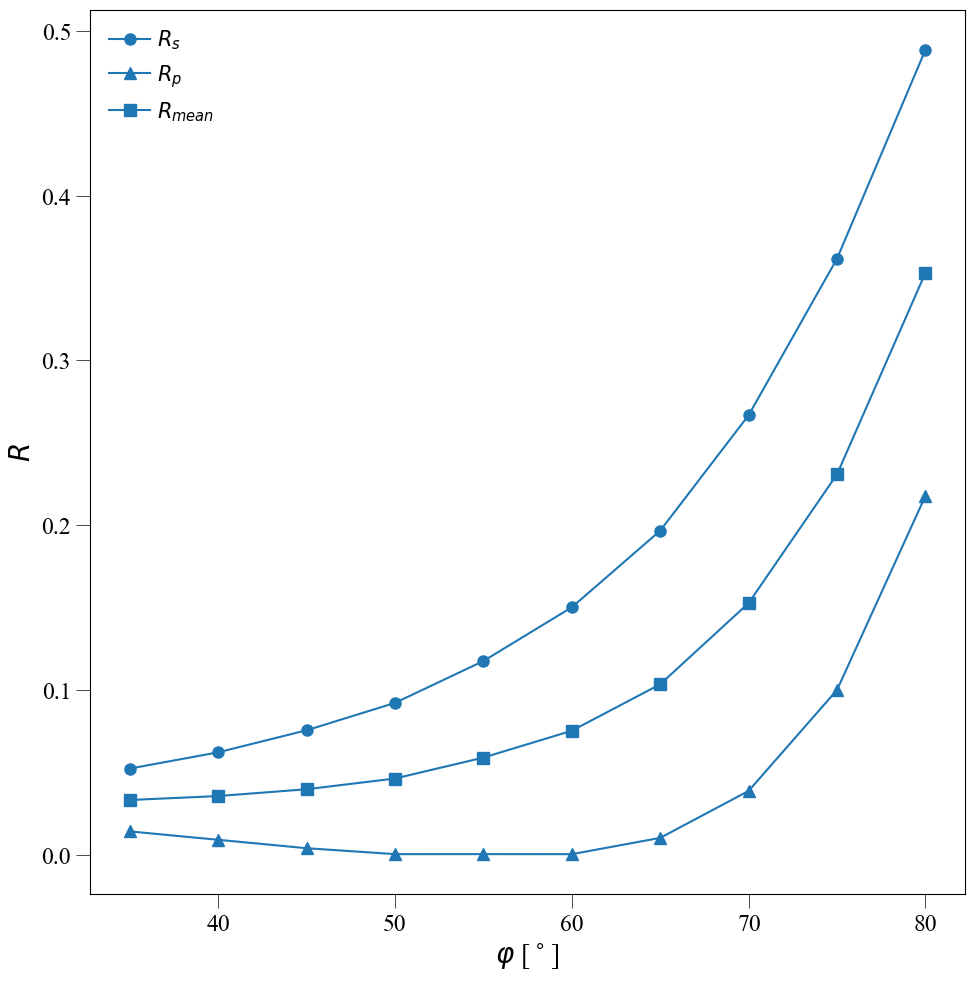
\includegraphics[scale=0.3]{amplituda}
                \captionsetup{justification=centering, font=footnotesize}
                \captionof{figure}{Závislost amplitud polarizovaného světla $R_s$, $R_p$ a $R$ na úhlu lomu $\varphi$.}
                \label{fig:amplituda}
                \raggedright
                \vspace{10pt}
                \par Pro zjištění Brewsterova úhlu byla provedena měření intenzit $I_s^R$ a $I_p^R$ v okolí $\varphi_0$, v němž bylo změřeno minimum amplitudy polarizovaného světla $R_p$. Údaje z měření jsou uvedeny v tabulce (3).
                \par Odtud je patrné, že minimum vyzařování nastává pod úhlem $\varphi_B$: 
                \begin{center}
                    $\varphi_B$ = 56.0(1)$^o$
                \end{center}
                Pak podle vzorce (5) zjistíme index lomu $n$: 
                \begin{center}
                    $n$ = 1.483(2)
                \end{center}
    \end{minipage}
    \hspace{10pt}  
    \begin{minipage}[t]{0.5\textwidth} 
                \par \centering
                \begin{tabular}{|c|c|c|c|}
                    \hline
                    $\varphi$ [$^o$] &  $I_s^R$ [V]  & $I_p^R$ [V] \\
                    \hline
                    60 & 8.713 & 0.219 \\
                    \hline
                    59 & 8.282 & 0.131 \\
                    \hline
                    58 & 7.876 & 0.071 \\
                    \hline
                    57 & 7.451 & 0.028 \\
                    \hline
                    56 & 7.109 & 0.014 \\
                    \hline
                    55 & 6.778 & 0.017 \\
                    \hline
                    54 & 6.398 & 0.039 \\
                    \hline
                    53 & 6.179 & 0.070 \\
                    \hline
                    52 & 5.871 & 0.122 \\
                    \hline
                    51 & 5.675 & 0.172 \\
                    \hline
                    50 & 5.431 & 0.242 \\
                    \hline
                \end{tabular}
                \captionsetup{justification=centering, font=footnotesize}
                \captionof{table}{Intenzity $I_s^R$ a $I_p^R$ v okolí $\varphi_0$.}
                \vspace{10pt}
                \raggedright
                \vspace{10pt}
                \par Ze vzorců (6) a (7) můžeme zjistit hodnoty indexu lomu pro úhly blízké Brewsterovu uhlu:  
                \vspace{10pt}
                \par \centering
                \begin{tabular}{|c|c|c|c|c}
                    \hline
                    $\varphi$ [$^o$] & $R_s$ & $R_p$ & $n$\\
                    \hline
                    45 & 0.075462 & 0.003875 & 1.410969 \\
                    \hline
                    50 & 0.092093 & 0.000267 & 1.390504 \\
                    \hline
                    55 & 0.117505 & 0.000280 & 1.453508 \\
                    \hline
                    60 & 0.150137 & 0.000251 & 1.481401 \\
                    \hline
                    65 & 0.196664 & 0.010137 & 1.455738 \\
                    \hline
                    70 & 0.266773 & 0.038669 & 1.451090 \\
                    \hline
                \end{tabular}
                \captionsetup{justification=centering, font=footnotesize}
                \captionof{table}{Hodnoty intenzity nepolarizovaného světla $I$, amplitud polarizovaného světla $R_s$ a $R_p$, a odrazivosti nepolarizovaného světla $R$}
                \vspace{10pt}
                \raggedright
                \par Odtud získáme průměrnou hodnotu $n$: 
                \begin{center}
                    $n$ = 1.42(3)
                \end{center}
                Budeme uvažovat index lomu $n_0$ rovný dříve získané hodnotě $n$ = 1.42(3). Pak podle vzorce (10) zjistíme hodnotu úhlu odrazu $\varphi_1$ a podle vzorců (8) a (9) zjistíme teoretické hodnoty hodnot odrazivosti $R_s$ a $R_p$: 
                \par \centering
                \vspace{10pt}
                \begin{tabular}{|c|c|c|c|c|c}
                    \hline
                    $\varphi_0$ [$^o$] & $\varphi_1$ [$^o$] &  $R_{s,teor}$  & $R_{p,teor}$ & $R_{teor}$\\
                    \hline
                    35 & 22.761 & 0.063 & 0.019 & 0.041 \\
                    \hline
                    40 & 25.694 & 0.074 & 0.013 & 0.043 \\
                    \hline
                    45 & 28.486 & 0.088 & 0.008 & 0.048 \\
                    \hline
                    50 & 31.111 & 0.107 & 0.003 & 0.055 \\
                    \hline
                    55 & 33.540 & 0.134 & 0.000 & 0.067 \\
                    \hline
                    60 & 35.742 & 0.170 & 0.002 & 0.086 \\
                    \hline
                    65 & 37.684 & 0.221 & 0.014 & 0.117 \\
                    \hline
                    70 & 39.333 & 0.292 & 0.043 & 0.168 \\
                    \hline
                    75 & 40.657 & 0.392 & 0.108 & 0.250 \\
                    \hline
                    80 & 41.626 & 0.532 & 0.238 & 0.385 \\
                    \hline
                \end{tabular}
                \captionsetup{justification=centering, font=footnotesize}
                \captionof{table}{Hodnoty intenzity nepolarizovaného světla $I$, amplitud polarizovaného světla $R_{s,teor}$, $R_{p,teor}$ a odrazivosti nepolarizovaného světla $R_{teor}$.}
                \vspace{10pt}
                \raggedright
    \end{minipage}
\newpage
    \begin{minipage}[t]{0.5\textwidth} 
                % \vspace{-212pt}
                Získáme tedy graf závislosti teoreticky vypočtených hodnot amplitud intenzit a porovnáme je s naměřenými hodnotami: 
                \par \centering
                \vspace{10pt}
                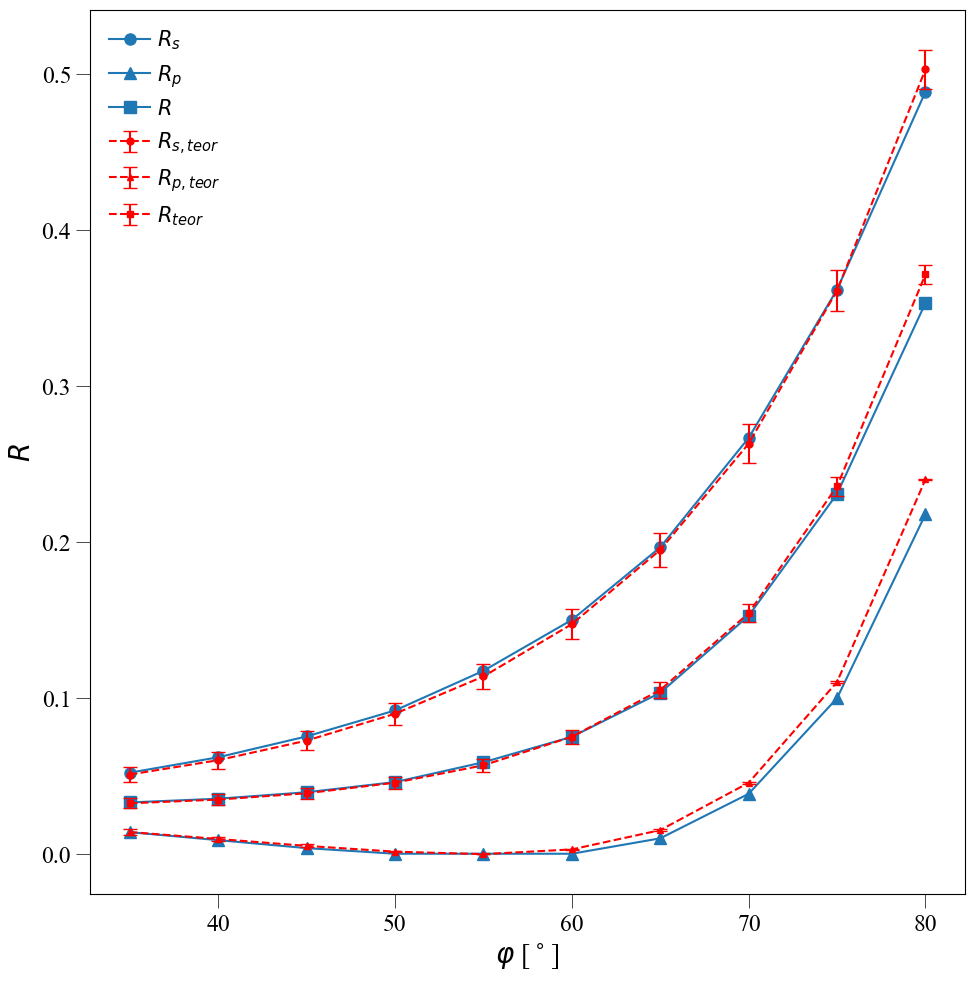
\includegraphics[scale=0.3]{amplituda_2}
                \captionsetup{justification=centering, font=footnotesize}
                \captionof{figure}{Závislost teoreticky vypočtených $R_{s,teor}$, $R_{p,teor}$ a $R_{teor}$ na úhlu lomu $\varphi$.}
                \label{fig:amplituda_2}
                \raggedright
                \vspace{10pt}
            \subsection{Průchod světla plexisklem a sklem}
                Dále jsme změřili rozměry paralelní desky, úhel dopadu $\alpha$ a výchylky detektoru $x$.
                \par Z výpočtů vyplývá: 
                \begin{center}
                    $d$ = 10.19(8) [mm]
                \end{center}
                \par Dále jsme vypočítali index lomu $n$ podle vzorce (16) a vypočítali teoretickou hodnotu výchylky detektoru $x_{teor}$ podle vzorce (16). Výsledky výpočtů jsou uvedeny v tabulce (6):
                \par \centering
                \vspace{10pt}
                \begin{tabular}{|c|c|c|c|c}
                    \hline
                    $\alpha$ [$^o$] & $x$ [mm] &  $n$  & $x_{teor}$ [mm]\\
                    \hline
                    5  & 0.31  & 1.533(6)  & 0.26(1) \\
                    \hline
                    10 & 0.61  & 1.513(6)  & 0.53(2) \\
                    \hline
                    15 & 0.90  & 1.489(6)  & 0.81(4) \\
                    \hline
                    20 & 1.24  & 1.498(6)  & 1.11(5) \\
                    \hline
                    25 & 1.59  & 1.497(6)  & 1.42(6) \\
                    \hline
                    30 & 1.96  & 1.493(6)  & 1.77(7) \\
                    \hline
                    35 & 2.36  & 1.489(7)  & 2.15(8) \\
                    \hline
                    40 & 2.84  & 1.497(7)  & 2.58(9) \\
                    \hline
                    45 & 3.34  & 1.495(8)  & 3.06(1) \\
                    \hline
                    50 & 3.95  & 1.510(9)  & 3.60(1) \\
                    \hline
                    53 & 4.27  & 1.497(9)  & 3.96(1) \\
                    \hline
                \end{tabular}
                \captionsetup{justification=centering, font=footnotesize}
                \captionof{table}{Úhel dopadu $\alpha$, výchylka detektoru $x$, index lomu $n$ a výchylka detektoru $x_{teor}$}
                \vspace{10pt}
                \raggedright
                \par Z toho vyplývá, že hodnota indexu lomu $n$ bude rovna:
                \begin{center}
                    $n_{teor}$ = 1.501(7)
                \end{center}
    \end{minipage}
    \hspace{10pt}
    \begin{minipage}[t]{0.5\textwidth} 
                Získané hodnoty $x$ a $x_{teor}$ jsou vyneseny v závislosti na úhlu dopadu $\alpha$, což je vidět na obrázku (\ref{fig:alpha}). 
                \par \centering
                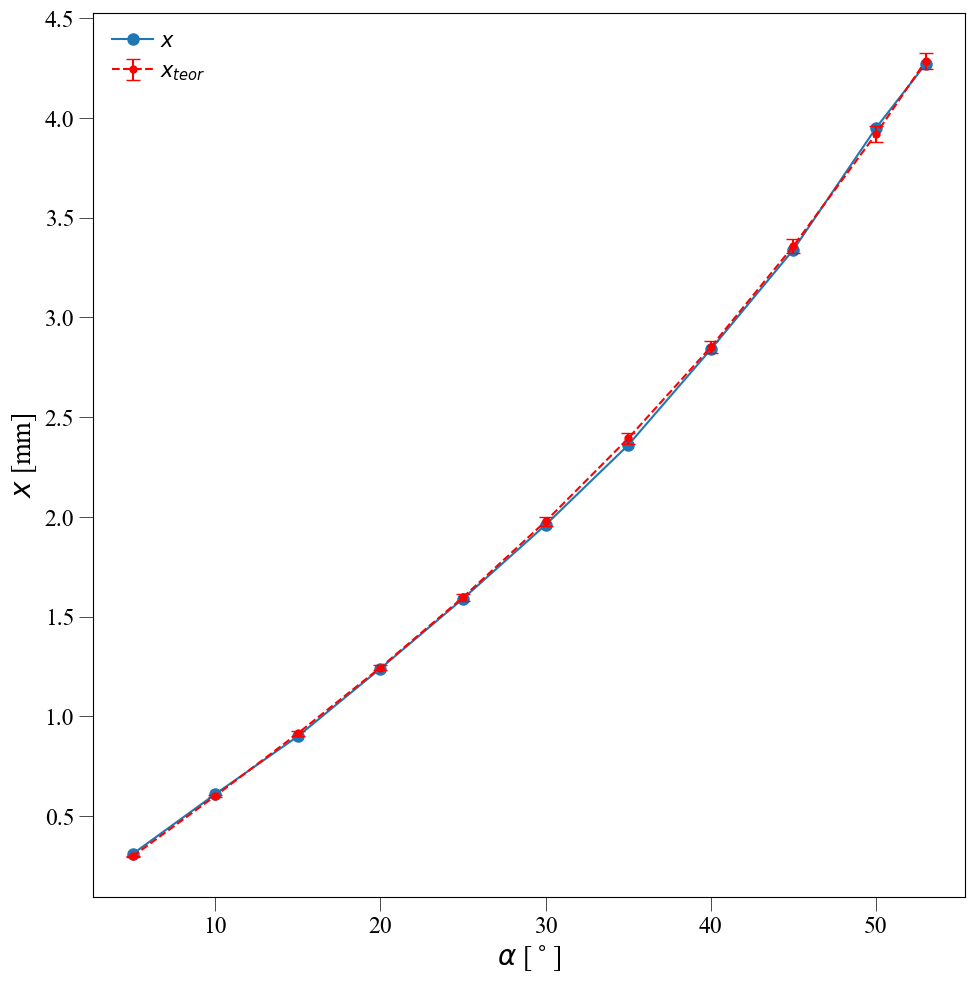
\includegraphics[scale=0.3]{alpha}
                \captionsetup{justification=centering, font=footnotesize}
                \captionof{figure}{Závislost $x$ a $x_{teor}$ na úhlu dopadu $\alpha$.}
                \label{fig:alpha}
                \vspace{10pt}
                \raggedright
                \vspace{10pt}
                \par K výpočtu veličin a jejich nejistot byla použita knihovna Uncertinties pro Python: \href{pypi.org/project/uncertainties}. Kód je přiložen k protokolu. 
        \section{Závěr}  
            \subsection{Odraz a lom světla}
                Z výpočtů vyplynula následující hodnota Brewsterova úhlu $\varphi_B$ = 56.0(1)$^o$. Poté jsme získali hodnoty indexu lomu $n$ = 1.483(2) z minima intenzity v $P$ filtru a teoreticky vypočtené hodnoty indexu lomu v blízkosti Brewsterova úhlu $n$ = 1.42(3). Hodnoty se sbíhají ve dvou řádech, což může svědčit o přijatelné přesnosti měření. 
            \subsection{Průchod světla plexisklem a sklem}
                Index lomu získaný teoretickými výpočty z úhlu dopadu $n_{teor}$ = 1.501(7) se rovněž shoduje s dříve získanými výsledky $n$ = 1.483(2) a $n$ = 1.42(3). Naměřené hodnoty výchylky detektoru $x$ a jejich teoretické protějšky $x_{teor}$ se rovněž sbližují, jak je patrné z grafu na obrázku (4).
    \end{minipage}
\newpage
    \par K výpočtu chyb byl použit následující kód: 
    \begin{lstlisting}[language=Python, basicstyle=\tiny, breaklines=true, postbreak=\mbox{\textbackslashspace}]
        #Importing the libraries

        import matplotlib.pyplot as plt
        import numpy as np
        import pandas as pd
        from scipy import stats
        from scipy.optimize import curve_fit
        import uncertainties as u 
        from uncertainties import ufloat
        from uncertainties.umath import *
        from uncertainties import unumpy

        # Constants, values and formulas for transformations

        I_0_s = 2.188*10**(3) #mV
        I_0_p = 3.788*10**(3) #mV
        
        d = ufloat(10.193, 0.0785854100114435) #m
        
        radians = np.pi/180
        degrees = 180/np.pi

        #Reading data

        data = pd.read_excel('data.xlsx')

        # Calculation 

        data['I_s'] = data['I_s']
        data['I_p'] = data['I_p']
        
        data['I_mean'] = (data['I_s'] + data['I_p']) / 2 
        
        data['R_s'] = data['I_s'] / I_0_s
        data['R_p'] = data['I_p'] / I_0_p
        
        data['R_mean'] = (data['R_s'] + data['R_p']) / 2
        
        phi_b = ufloat(data['phi_min'][4], 0.1)
        
        n = ufloat(np.tan(np.radians(phi_b.nominal_value)), np.tan(np.radians(phi_b.std_dev)))
        
        print('n =', n)
        
        data['n_under'] = np.sqrt(((1+np.sqrt(data['R_s'][2:5]))*(1+np.sqrt(data['R_p'][2:5])))/((1-np.sqrt(data['R_s'][2:5]))*(1-np.sqrt(data['R_p'][2:5]))))
        data['n_up'] = np.sqrt(((1+np.sqrt(data['R_s'][5:8]))*(1-np.sqrt(data['R_p'][5:8])))/((1-np.sqrt(data['R_s'][5:8]))*(1+np.sqrt(data['R_p'][5:8]))))
        
        n_mean = ufloat(np.mean(np.array(data['n_under'][2:5],data['n_up'][5:8])), np.std(np.array(data['n_under'][2:5],data['n_up'][5:8])))
        
        print('n_mean =', n_mean)
        
        phi_1 = []
        for ii,ID in enumerate(data['phi']):
            phi_1.append(degrees *(asin(sin(radians * (data['phi'][ii]))/n_mean)))
        data['phi_1'] = phi_1
        
        R_s_1 = []
        for ii,ID in enumerate(data['phi']):
            R_s_1.append(np.abs(-1*sin(radians * (data['phi'][ii]-data['phi_1'][ii])) / sin(radians * (data['phi'][ii]+data['phi_1'][ii])))**2)
        data['R_s_1'] = R_s_1
        
        R_p_1 = []
        for ii,ID in enumerate(data['phi']):
            R_p_1.append(np.abs(-1*tan(radians * (data['phi'][ii]-data['phi_1'][ii])) / tan(radians * (data['phi'][ii]+data['phi_1'][ii])))**2)
        data['R_p_1'] = R_p_1
        
        data['R_mean_1'] = (data['R_s_1'] + data['R_p_1']) / 2
        
        n_2 = []
        for ii,ID in enumerate(data['alpha']):
            n_2.append(sqrt(sin(radians*np.array(data['alpha'][ii]))**2 + (1 - (data['x_1'][ii] / (d*sin(radians*data['alpha'][ii]))))**(-2)*np.cos(radians*data['alpha'][ii])**2))
        data['n_2'] = n_2
        
        x_teor = []
        for ii,ID in enumerate(data['alpha']):
            # x_teor.append((1 - np.cos(np.radians(data['alpha'][ii])) / sqrt(n**2 - np.sin(np.radians(data['alpha'][ii]))**2)) * d * np.sin(np.radians(data['alpha'][ii])))
            # x_teor.append((1 - np.cos(np.radians(data['alpha'][ii])) / sqrt(n_mean**2 - np.sin(np.radians(data['alpha'][ii]))**2)) * d * np.sin(np.radians(data['alpha'][ii])))
             x_teor.append((1 - np.cos(np.radians(data['alpha'][ii])) / sqrt(n_2_mean**2 - np.sin(np.radians(data['alpha'][ii]))**2)) * d * np.sin(np.radians(data['alpha'][ii])))
        data['x_teor'] = x_teor
        
        n_2_val = []
        n_2_err = []
        
        for ii,ID in enumerate(data['n_2']):
            n_2_val.append(data['n_2'][ii].nominal_value)
            n_2_err.append(data['n_2'][ii].std_dev)
        
        n_2_mean = ufloat(np.mean(np.array(n_2_val)), np.sqrt(np.std(np.array(n_2_err))**2+np.mean(np.array(n_2_err))**2))
        
        print('n_2_mean =', n_2_mean)
        
        # print(data)
    \end{lstlisting}        
\end{document}